\documentclass[12pt,a4paper]{article}
\usepackage[a4paper,top=3cm,bottom=3.5cm,left=3cm,right=3cm,marginparwidth=1.75cm]{geometry}
\usepackage[bottom]{footmisc} 
\usepackage[table]{xcolor} % KEEP THIS FIRST OR LATEX BORKS
\usepackage[utf8]{inputenc}
\usepackage{csquotes}
\usepackage{graphicx} % Required for inserting images
\usepackage[french]{babel}
\usepackage[T1]{fontenc}
\usepackage[sorting=none]{biblatex}
\addbibresource{biblio.bib}
\usepackage{cryptocode}
\usepackage{booktabs}
\setlength\heavyrulewidth{0.20ex}
\setlength\cmidrulewidth{0.10ex}
\setlength\lightrulewidth{0.10ex}
\usepackage{multirow}
\usepackage{array}
\usepackage{float}
\usepackage{setspace}
\usepackage[skip=13pt, indent=20pt]{parskip}
\usepackage[colorlinks=true, allcolors=blue]{hyperref} %autoref
\usepackage{titlesec}
\setlength\headheight{28pt}
\titlespacing*{\section}{0pt}{5mm}{5mm}
\titlespacing*{\subsection}{0pt}{5mm}{5mm}
\titlespacing*{\subsubsection}{0pt}{4mm}{4mm}
\usepackage{tikz}
\usepackage{enumitem}
\usepackage{pifont}
\usepackage{changepage,threeparttable} % for wide tables
\usepackage{svg}
\usepackage{listings}
\usepackage{pkg/msc}
\usepackage{pgfgantt}
\usepackage[ingenieur]{pkg/coverinsa}
\usepackage[most]{tcolorbox}
\usepackage{xcolor}
\tcbset{
  colback=gray!5,
  colframe=black!80,
  boxrule=0.5pt,
  arc=2mm,
  left=2mm,
  right=2mm,
  top=1mm,
  bottom=1mm,
  fonttitle=\bfseries,
  coltitle=white
}

\auteur{Salah AL-BAKRI}{}
\titre{INTITULE DU PFE }
\entreprisenom{ Orange Cyberdefense }
\tuteur{Rémi ABIVEN}{}
\entrepriselogo{}{assets/ocd-logo-original.png}{3cm}
\anneeuniversitaire{2025-2026}
\correspondantINSA{Muriel}{PRESSIGOUT}
\pfesoutenule{XX/06/2026}

\lstdefinestyle{goStyle}{
  language=Go,
  backgroundcolor=\color{white},
  basicstyle=\ttfamily\footnotesize,
  keywordstyle=\color{red},
  commentstyle=\color{blue},
  stringstyle=\color{red},
  numbers=left,
  numberstyle=\tiny\color{gray},
  stepnumber=1,
  numbersep=5pt,
  showstringspaces=false,
  breaklines=true
}

% default
\lstset{
  language=Go,
  tabsize=4,
  backgroundcolor=\color{white},
  basicstyle=\ttfamily\footnotesize,
  keywordstyle=\color{red},
  commentstyle=\color{blue},
  stringstyle=\color{red},
  numbers=left,
  numberstyle=\tiny\color{gray},
  stepnumber=1,
  numbersep=5pt,
  showstringspaces=false,
  breaklines=true
}
\lstdefinestyle{bashStyle}{
  language=Bash,
  tabsize=4,
  backgroundcolor=\color{white},
  basicstyle=\ttfamily\footnotesize,
  keywordstyle=\color{blue},
  commentstyle=\color{green},
  stringstyle=\color{red},
  numbers=left,
  numberstyle=\tiny\color{gray},
  stepnumber=1,
  numbersep=5pt,
  showstringspaces=false,
  breaklines=true
}

\lstdefinelanguage{YAML}{
  keywords={true,false,null,yes,no},
  keywordstyle=\color[HTML]{3dad5d}\bfseries,
  sensitive=false,
  comment=[l]{\#},
  morecomment=[l]{\#},
  commentstyle=\color{gray}\itshape,
  stringstyle=\color[HTML]{95cede},
  morestring=[b]",
  morestring=[b]',
}

\lstdefinestyle{yamlStyle}{
  language=YAML,
  basicstyle=\ttfamily\footnotesize,
  keywordstyle=\color[HTML]{3dad5d},
  morekeywords={[2]true,false,null, p2p, rdvp, maddr, static-relays},
  keywordstyle={[2]\color[HTML]{3dad5d}},
  commentstyle=\color{gray},
  stringstyle=\color{black},
  numbers=left,
  numberstyle=\tiny\color{gray},
  stepnumber=1,
  numbersep=6pt,
  showstringspaces=false,
  breaklines=true,
  rulecolor=\color{gray!40},
  alsoletter=-,
}

\renewcommand{\sectionautorefname}{Section}
\renewcommand{\subsectionautorefname}{Section}
\renewcommand{\subsubsectionautorefname}{Section}


\begin{document}

\setstretch{1}

\maketitle
\pagebreak


\thispagestyle{empty}
\setcounter{tocdepth}{2}


\pagebreak



\setcounter{page}{1}


% Inclure la section "Autorisation de diffusion et d’archivage du rapport"
\addcontentsline{toc}{section}{Autorisation de diffusion et d’archivage du rapport}
\begin{center}
\textbf{\LARGE Autorisation de diffusion et d’archivage du rapport}
\end{center}

\subsection*{Informations de l’auteur}
\begin{itemize}[label={--}]
    \item NOM et Prénom de l’auteur : \underline{\hspace{5cm}}
    \item Spécialité : \underline{\hspace{5cm}}
    \item Titre du projet : \underline{\hspace{5cm}}
    \item Nom de l’entreprise : \underline{\hspace{5cm}}
    \item NOM et Prénom du tuteur du Projet de Fin d'Études : \underline{\hspace{5cm}}
    \item NOM et Prénom du correspondant pédagogique INSA : \underline{\hspace{5cm}}
\end{itemize}

\section*{Archivage du rapport de PFE}
À l'issue de son stage, l'étudiant(e) stagiaire rédigera un rapport qui devra être communiqué aussi bien à l'organisme d'accueil qu'à l'établissement d'enseignement supérieur pour évaluation.  
Par obligation réglementaire (instruction 2005-003 parue au B.O du 16 juin 2005), l’INSA de Rennes est tenu de conserver pour archive une version du rapport de PFE. Tout rapport de PFE sera donc systématiquement archivé par le département de l'auteur de l’INSA de Rennes.   
Si le rapport contient des données confidentielles, une version expurgée pourra être archivée à la place de la version intégrale.

\begin{itemize}
    \item ☐ archivage de la version intégrale
    \item ☐ archivage de la version expurgée, merci de justifier : \underline{\hspace{5cm}}
\end{itemize}

\section*{Diffusion du rapport de PFE}
\subsection*{Autorisation de diffusion par l’entreprise commanditaire}
Nous, soussignés, représentant de l’entreprise commanditaire :  
\begin{itemize}[label={--}]
    \item Nom : \underline{\hspace{5cm}}
    \item Prénom : \underline{\hspace{5cm}}
    \item Fonction : \underline{\hspace{5cm}}
\end{itemize}

\begin{itemize}
    \item ☐ autorisons le signalement et la diffusion du document désigné ci-dessus sur l’intranet du département de l'auteur de l’INSA
    \item ☐ autorisons uniquement le signalement du document désigné ci-dessus sur l’intranet du département de l'auteur de l’INSA
    \item ☐ n’autorisons ni le signalement ni la diffusion du document désigné ci-dessus sur l’intranet du département de l'auteur de l’INSA et demandons la confidentialité (5 ans maximum), jusqu’à la date suivante (mois/année) : \underline{\hspace{3cm}}
\end{itemize}

Fait à \underline{\hspace{3cm}}, le \underline{\hspace{3cm}} \\
Signature et/ou cachet de l’entreprise commanditaire : \underline{\hspace{5cm}}

\subsection*{Autorisation de diffusion par l’auteur}
Je soussigné(e), \\
Nom : \underline{\hspace{5cm}} \\
Prénom : \underline{\hspace{5cm}}

\begin{itemize}
    \item ☐ autorise le signalement et la diffusion du document désigné ci-dessus sur l’intranet du département de l'auteur de l’INSA
    \item ☐ autorise uniquement le signalement du document désigné ci-dessus sur l’intranet du département de l'auteur de l’INSA
    \item ☐ n’autorise ni le signalement ni la diffusion du document désigné ci-dessus sur l’intranet du département de l'auteur de l’INSA
\end{itemize}

Fait à \underline{\hspace{3cm}}, le \underline{\hspace{3cm}} \\
Signature : \underline{\hspace{5cm}}

\subsection*{Autorisation de diffusion par le correspondant pédagogique de l’INSA}
Par défaut, le correspondant pédagogique, membre de l’équipe enseignante, est supposé avoir une contribution mineure sur le rapport et ne pas s’opposer à sa diffusion. Merci de contacter le responsable des stages du département en cas d’opposition.



\pagebreak

% Inclure la section "Remerciements"
\addcontentsline{toc}{section}{Remerciements}
\section*{Remerciements}

Je souhaite adresser mes remerciements à mon tuteur de stage, M. Rémi Abiven, pour avoir partagé ses connaissances de manière pédagogique, pour sa disponibilité à répondre à mes questions et pour la qualité de son encadrement.

J’exprime également ma reconnaissance à M. Jean-Michel Auneau, manager de l’équipe Next Generation Firewall (au sein de laquelle j’ai effectué mon stage), pour m’avoir placé dans de bonnes conditions afin de mener à bien mon projet et pour le suivi attentif de l’avancement de l'alternance.

TODO ...

Je remercie l’ensemble des membres de l’équipe Next Gen. Firewall. 

J’aimerais également remercier ma responsable pédagogique, Mme. Muriel Pressigout, pour ses conseils lors de sa visite en entreprise.

Enfin, je remercie toute l’équipe pédagogique de l’INSA Rennes pour la qualité de son enseignement, qui m’a permis d’acquérir les compétences nécessaires à la réussite de cet alternance.
\pagebreak

% Ajoutez ici la section "TABLE DES MATIERES."
\addcontentsline{toc}{section}{Table des matières}
\tableofcontents
\newpage

% Ajoutez ici la section "Glossaire."
\addcontentsline{toc}{section}{Glossaire}
\section*{Glossaire}

Le glossaire permet de centraliser des termes et abréviations utilisées dans le document. Il est facultatif, mais recommandé si votre document comprend beaucoup de jargon. Attention, même si une abréviation apparaît dans le glossaire, il faut la définir la première fois que vous l’utilisez.

Exemple :

INSA : Institut national des sciences appliquées

PFE : Projet de fin d’études

\pagebreak

\section{Introduction}
Durant mes trois années d’études au sein du département informatique de l'INSA Rennes, je me suis particulièrement intéressé à la cybersécurité, tant dans ses aspects applicatifs qu'infrastructurels. J’ai choisi l’option sécurité lors du deuxième semestre de ma première année, ce qui m’a permis d’acquérir de solides connaissances dans ce domaine à travers des enseignements tels que : sécurité offensive, sécurité des réseaux, programmation sécurisée et cryptographie.

Pour valider ma dernière année du cycle d’ingénieur, j’ai opté pour un contrat de professionnalisation incluant un projet de fin d’études (PFE) tout au long de l’année. J’ai ainsi eu l’opportunité de réaliser cette alternance au sein de l’entreprise Orange Cyberdefense, en tant qu’ingénieur sécurité dans l’équipe Next Generation Firewall. Cette expérience m’a permis de développer davantage mes compétences et de renforcer mes connaissances dans le domaine qui me passionne.

Ce rapport présente les objectifs et les travaux réalisés durant cette période d’alternance. Dans un premier temps, je présenterai l’entreprise Orange Cyberdefense, suivie d’une description du contexte dans lequel s’est déroulé l'alternance. Je décrirai ensuite le (TODO). Par la suite, j’aborderai en détail les missions effectuées, les difficultés rencontrées ainsi que les solutions mises en œuvre. Enfin, je conclurai par une synthèse des principaux éléments abordés dans ce rapport.
\pagebreak

\section{Présentation de l'entreprise}

\subsection{Histoire}
Orange Cyberdefense est une entreprise française leader européen de la cybersécurité, proposant des services de protection, de détection et de réponse aux cybermenaces. L'entreprise s'est construite progressivement à partir des expertises en sécurité du groupe Orange, avant de connaître une accélération majeure avec des acquisitions stratégiques.

Les premières activités de cybersécurité d'Orange remontent aux années 2000, lorsque l'opérateur développe ses capacités internes de protection des infrastructures et des données. En 2016, Orange structure officiellement sa division cybersécurité sous la marque Orange Cyberdefense.

L'année 2019 marque un tournant décisif avec l'acquisition de Securelink, leader européen des services managés de cybersécurité. Cette opération permet à Orange Cyberdefense de devenir l'un des principaux acteurs européens du secteur, en intégrant plus de 1 000 experts en sécurité.

Orange Cyberdefense connaît une croissance soutenue avec une expansion internationale continue. L'entreprise compte aujourd'hui plus de 3 000 experts répartis dans plus de 20 pays et protège plus de 2 000 organisations à travers le monde.

La figure suivante montre la présence de l’entreprise dans le monde 

\begin{figure}[H]
\centering
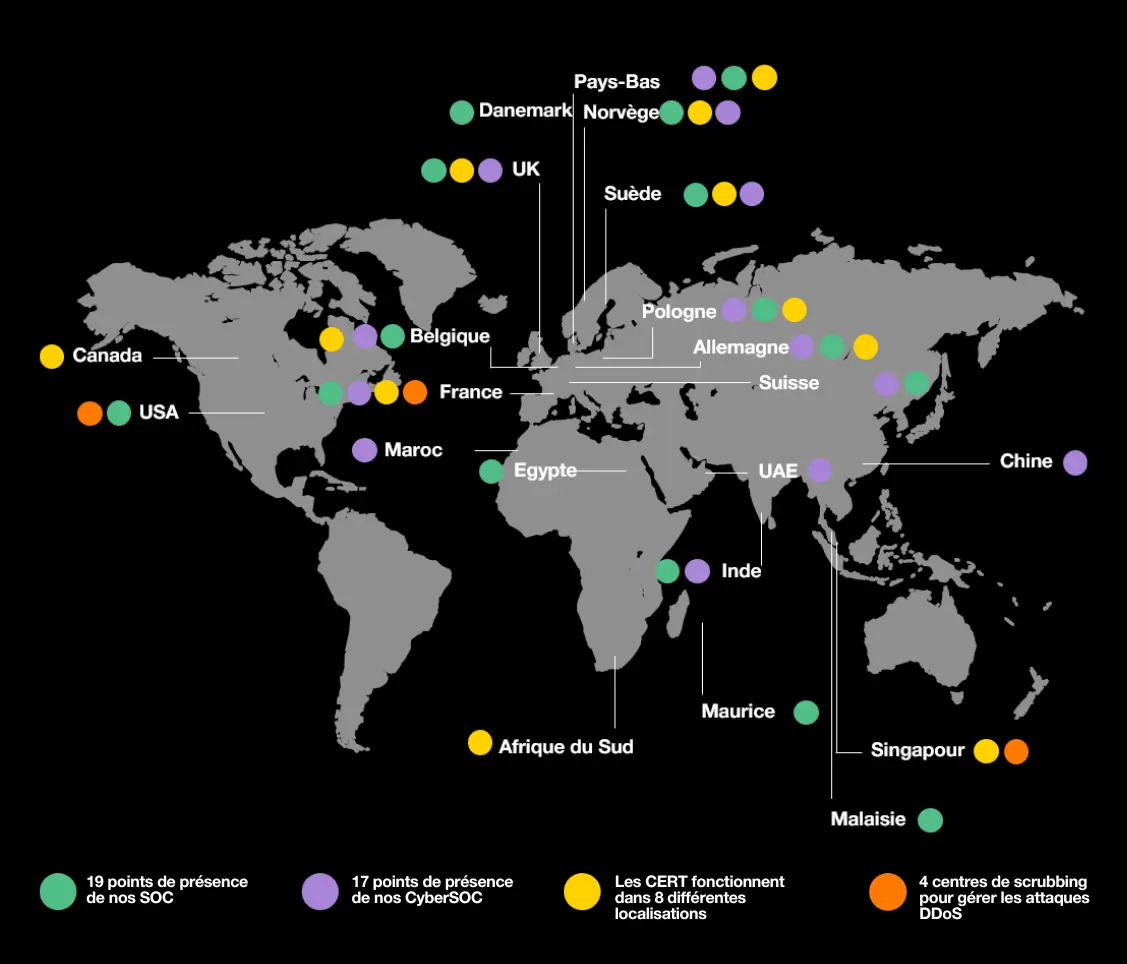
\includegraphics[width=0.7\textwidth]{assets/OCD_world.png}
\caption{Présence d'Orange Cyberdefense dans le monde}
\end{figure}

\subsection{Services et Produits}
L'entreprise structure son offre autour du cycle de vie complet de la cybersécurité : anticiper, identifier, protéger, détecter et répondre. Elle propose ainsi des services de conseil et gestion des risques, d'audit et tests d'intrusion, de détection et réponse aux incidents via un réseau mondial de SOC, ainsi que de gestion des vulnérabilités.\footnote{L'entreprise propose un large gamme de services en cybersécurité. Dans le cadre de cette alternance, je présente uniquement les services en lien direct avec ma mission.}

\subsubsection{L'Unified Managed Firewall (UMFW)}

Parmi ces services, l'Unified Managed Firewall (UMFW) occupe une place centrale. Il s'agit d'un service managé de pare-feu, qui assure la protection en continu des réseaux des clients contre les intrusions et attaques externes. Le MFW permet de filtrer le trafic, d'appliquer des politiques de sécurité adaptées et de détecter les comportements suspects en temps réel, tout en déchargeant les équipes internes des clients de la gestion quotidienne de cette protection.

Pour couvrir les besoins variés de ses clients, Orange Cyberdefense s'appuie sur plusieurs technologies de pare-feu de référence, notamment \textit{Fortinet}, \textit{Check Point} et \textit{Palo Alto Networks}. Chaque technologie est sélectionnée selon le contexte et les exigences de l'environnement du client.

Dans ce cadre, mon alternance s'inscrit au sein de l'équipe d'expertise \textit{Check Point}, en charge de la gestion et de l'administration des solutions de pare-feu Check Point déployées chez les clients d'Orange Cyberdefense.

\subsection{Structure de l'entreprise}
TODO : mentionner que nous somme dans la 2eme BU et dnas le GOPS

TODO : mentionner qu'il y les expert et les devs dans l'équipe

TODO : mon positionnement dans l'équipe
\pagebreak

\section{Contexte et objectifs de l'alternance}

% Dans ton cas, celui-ci serait la nécessité de sécurité renforcée des applications déployées à l'échelle nationale, ou quelque chose de ce type. Tu expliques ensuite ce que tu vas faire dans ce contexte général (tester et renforcer la sécurité de l'application Cyclades, avec tels et tels objectifs précis (ce que tu as bien décrit))

\pagebreak

\section{Mise en place et exploitation du laboratoire de tests}

\subsection{Objectifs du laboratoire}

Le laboratoire de tests a été mis en place afin de reproduire une
infrastructure Check Point représentative d’un environnement de
production. Il permet d’expérimenter le déploiement et
l’administration des différents composants de sécurité tout en
analysant leur comportement dans plusieurs scénarios
d’exploitation.

Plus précisément, ce laboratoire vise à :

\begin{itemize}
    \item étudier l’architecture Check Point et ses mécanismes de gestion ;
    \item expérimenter l’architecture \textit{Multi-Domain Manager} ;
    \item analyser le processus de déploiement des politiques de sécurité ;
    \item observer les mécanismes de haute disponibilité via le clustering.
\end{itemize}

L’infrastructure a été déployée dans un environnement virtualisé
afin de simuler plusieurs domaines de sécurité tout en conservant
une architecture proche de celle rencontrée dans des
environnements réels.

%------------------------------------------------

\subsection{Architecture générale du laboratoire}

Le laboratoire repose sur une architecture Check Point classique
composée de trois éléments principaux : une interface
d’administration, un serveur de management et une ou plusieurs
passerelles de sécurité. Ces composants interagissent selon un
modèle hiérarchique dans lequel les politiques de sécurité sont
définies par l’administrateur, centralisées sur un serveur de
management puis déployées vers les passerelles chargées
d’inspecter le trafic réseau.

La figure~\ref{fig:archi_lab} illustre l’organisation générale de
cette architecture. Les différents composants y sont numérotés
afin de faciliter leur identification dans les descriptions
suivantes.

\begin{figure}[H]
    \centering
    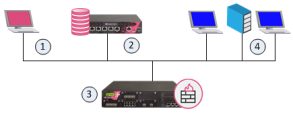
\includegraphics[width=0.75\textwidth]{assets/archi_ckp.png}
    \caption{Architecture générale du laboratoire}
    \label{fig:archi_lab}
\end{figure}

\paragraph{SmartConsole (1).}

La \textbf{SmartConsole} constitue l’interface graphique
d’administration de l’environnement Check Point. Elle permet à
l’administrateur de définir les politiques de sécurité, de gérer
les objets réseau et d’analyser les journaux d’événements.

La SmartConsole ne stocke aucune configuration localement. Toutes
les actions effectuées par l’administrateur sont transmises au
serveur de management via un canal sécurisé appelé
\textit{Secure Internal Communication} (SIC).

\paragraph{Serveur de management (2).}

Le serveur de management constitue le cœur du système de gestion.
Il centralise l’ensemble des politiques de sécurité, la base
d’objets réseau ainsi que les journaux d’événements.

Dans l’architecture du laboratoire, ce rôle est assuré par un
\textbf{Multi-Domain Manager} (MDM). Ce composant permet
d’administrer plusieurs domaines de sécurité indépendants à
partir d’une plateforme unique.

Les politiques de sécurité définies dans la SmartConsole sont
compilées par le serveur de management puis déployées vers les
passerelles via l’opération \textit{Install Policy}.

\paragraph{Security Gateway (3).}

La \textbf{Security Gateway} est l’équipement chargé d’inspecter
le trafic réseau. Positionnée en coupure sur le réseau, elle
applique les politiques de sécurité reçues depuis le serveur de
management et analyse les flux en temps réel.

\paragraph{Environnement à protéger (4).}

L’environnement à protéger représente l’ensemble des ressources
internes du réseau : postes de travail, serveurs et services
applicatifs. Dans le cadre du laboratoire, cet environnement
simule un périmètre client afin d’observer le comportement des
passerelles de sécurité dans des conditions proches d’un
environnement réel.

%------------------------------------------------

\subsection{Architecture Multi-Domain Manager}

Afin de reproduire un environnement multi-client, le laboratoire
s’appuie sur l’architecture \textbf{Multi-Domain Manager} (MDM)
proposée par Check Point \cite{checkpoint_mds_r8030}.

Le Multi-Domain Manager constitue le serveur central de
management. Il permet d’administrer simultanément plusieurs
domaines de sécurité indépendants à partir d’une plateforme
unique. L’administrateur s’y connecte via la SmartConsole afin
de superviser les différents domaines, gérer les objets globaux,
administrer les comptes utilisateurs et consulter les journaux
centralisés.

Cette architecture permet de gérer plusieurs domaines de sécurité
indépendants depuis un point d’administration centralisé. Chaque
domaine dispose de ses propres politiques de sécurité, de ses
objets réseau et de ses passerelles, tout en restant isolé des
autres domaines.

La figure~\ref{fig:mds_overview} illustre l’organisation générale
d’un déploiement multi-domaine.

\begin{figure}[H]
    \centering
    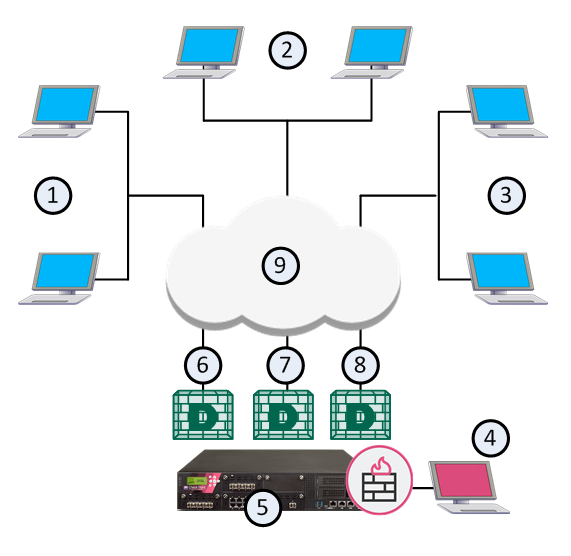
\includegraphics[width=0.75\textwidth]{assets/mds_overview.png}
    \caption{Architecture générale du laboratoire}
    \label{fig:mds_overview}
\end{figure}


\subsubsection{Customer Management Add-on / Domain Management Server}

Au sein du Multi-Domain Manager, chaque domaine est administré
par un \textbf{Domain Management Server} (DMS), historiquement
appelé \textbf{Customer Management Add-on} (CMA).

Chaque DMS constitue un serveur de management autonome,
équivalent à un Security Management Server dans une architecture
mono-domaine.

Il administre de manière indépendante :

\begin{itemize}
    \item les politiques de sécurité et les règles NAT ;
    \item les objets réseau du domaine ;
    \item les Security Gateways associées ;
    \item les journaux et paramètres propres au domaine.
\end{itemize}

Cette séparation garantit qu’un administrateur d’un domaine ne
peut accéder ni aux données ni aux politiques d’un autre domaine,
ce qui est particulièrement important dans les environnements
multi-clients.

%------------------------------------------------

\subsection{Déploiement des passerelles de sécurité}

Les politiques définies dans les différents Domain Management
Servers sont déployées vers les passerelles de sécurité
associées. Ces équipements constituent les éléments chargés
d’appliquer effectivement les règles de sécurité sur le trafic
réseau.

\subsubsection{Security Gateway}

Une \textbf{Security Gateway} est un équipement positionné en
coupure sur le réseau qui reçoit la politique compilée depuis
son serveur de management. Elle inspecte ensuite le trafic en
temps réel afin de déterminer si les communications doivent être
autorisées ou bloquées.

Les journaux générés lors de l'inspection du trafic sont
ensuite envoyés vers le serveur de management afin d’être
analysés dans la SmartConsole.

\subsubsection{Déploiement en cluster}

Afin de garantir la continuité de service, les Security Gateways
peuvent être déployées en \textbf{cluster} grâce à la technologie
\textbf{ClusterXL} de Check Point.

Un cluster regroupe plusieurs passerelles physiques qui partagent
une adresse IP virtuelle et fonctionnent comme un seul
équipement du point de vue du réseau et du serveur de management.

Dans un cluster classique à deux membres, les passerelles peuvent
se trouver dans les états suivants :

\begin{itemize}
    \item \textbf{Active} : la passerelle traite le trafic réseau ;
    \item \textbf{Standby} : la passerelle est synchronisée et prête
    à prendre le relais ;
    \item \textbf{Down} : la passerelle n’est plus opérationnelle.
\end{itemize}

En fonctionnement normal, seul le membre \textit{Active} traite le
trafic. En cas de défaillance  (\textit{failover}), le membre \textit{Standby} prend
automatiquement le relais, garantissant la
continuité du service sans interruption.

La figure~\ref{fig:cluster_states} illustre les états possibles d'un
cluster à deux membres.
 
\begin{figure}[H]
    \centering
    \begin{tikzpicture}[
        gwbox/.style  = {rectangle, draw, rounded corners=6pt,
                         minimum width=3.2cm, minimum height=1.2cm,
                         font=\small, align=center},
        vipbox/.style = {rectangle, draw=black!50, rounded corners=4pt,
                         minimum width=2.4cm, minimum height=0.8cm,
                         font=\footnotesize, align=center, fill=gray!10},
        arr/.style    = {->, >=stealth, thick},
        lbl/.style    = {font=\footnotesize}
    ]
        \node[vipbox] (vip) at (0, 3.2)
            {\textbf{IP virtuelle (VIP)}\\Adresse cluster};
        \node[gwbox, fill=teal!10] (cma) at (0, 5.0)
            {\textbf{CMA}\\Install Policy};
        \node[gwbox, fill=green!12] (gwa) at (-3.2, 1.2)
            {\textbf{Gateway 1}\\
             \textcolor{green!60!black}{\textbf{Active}}\\
             {\footnotesize Traite le trafic}};
        \node[gwbox, fill=orange!10] (gwb) at (3.2, 1.2)
            {\textbf{Gateway 2}\\
             \textcolor{orange!80!black}{\textbf{Standby}}\\
             {\footnotesize Synchronisé, en attente}};
        \node[gwbox, fill=gray!8] (net) at (0, -0.8)
            {\textbf{Réseau}\\Trafic entrant/sortant};
 
        \draw[arr, teal!60]  (cma)  -- node[right, lbl]{politique} (vip);
        \draw[arr, black!50] (vip)  -- (gwa);
        \draw[arr, black!50] (vip)  -- (gwb);
        \draw[<->, >=stealth, dashed, gray]
            (gwa.south east) -- node[below, lbl]{sync état} (gwb.south west);
        \draw[arr] (net.north) -- (vip.south);
    \end{tikzpicture}
    \caption{Security Gateway en cluster~: états Active et Standby}
    \label{fig:cluster_states}
\end{figure}

\pagebreak

\section{Projet Watchdog : Automatisation et monitoring}

\subsection{Contexte du projet}
Problématiques identifiées
Besoins clients et équipes de production
Objectifs du projet Watchdog


\subsection{Analyse des besoins et spécifications}
Cahier des charges
Fonctionnalités attendues
Contraintes techniques et opérationnelles


\subsection{Conception de la solution}
Architecture technique du Watchdog
Choix technologiques (API Checkpoint, langages de script)
Schéma de fonctionnement

\subsection{Développement et implémentation}
Utilisation des API Checkpoint
Développement des scripts de monitoring
Collaboration avec l'équipe de développement
Gestion des versions et du code

\subsection{Tests et validation}
Scénarios de tests du Watchdog
Tests en environnement de lab
Validation avec les équipes de production
\pagebreak

\input{src/10_a_suivre}
\pagebreak

\section*{ANNEXE A – patati patata}
\addcontentsline{toc}{section}{Annexe A – patati patata}

Votre rapport peut compter un nombre indéterminé d’annexes, numérotées A, B, C, qui ne sont pas décomptées dans le nombre de pages du rapport. Étant optionnelles, les évaluateurs peuvent ne pas les lire. C’est l’occasion de placer des documents qui rompraient la continuité du texte principal, tels que des résultats d’expériences de vérification, ou qui l’allongeraient trop. Par exemple, plutôt que de mettre trois graphes pour présenter les résultats sur trois échantillons différents, ce qui peut prendre 1.5 pages, on n’en conserve qu’un dans le texte principal pour présenter brièvement la méthode, ainsi qu’un tableau de synthèse, les courbes pour les deux autres échantillons étant renvoyées en annexe.



\section*{Annexe : Planning du stage par phases hebdomadaires}
\addcontentsline{toc}{section}{Annexe B - Planning de l'alternance}

Le stage s’est déroulé du \textbf{12 mai au 25 juillet 2025}, soit une durée totale de 11 semaines. Le tableau suivant présente la répartition hebdomadaire des différentes phases du stage:

\bigskip


\begin{ganttchart}[
    hgrid,
    vgrid,
    x unit=0.9cm,
    y unit title=0.7cm,
    y unit chart=0.9cm,
    bar height=0.7,
    bar/.style={fill=blue!30, rounded corners=3pt},
    milestone/.style={fill=orange!50},
    bar label font=\footnotesize\bfseries,
    milestone label font=\footnotesize\bfseries,
    group label font=\small\bfseries,
    title label font=\small\bfseries,
    group/.style={draw=black, fill=green!20, rounded corners=3pt},
    group height=0.5,
    group peaks={0}{0}{0.3},
    bar left shift=0.1,
    bar right shift=-0.1
]{1}{11}
\gantttitle{Semaines du stage}{11} \\
\gantttitlelist{1,...,11}{1} \\

\ganttgroup{Phase préparatoire}{1}{3} \\
\ganttbar{Accueil et cadrage}{1}{1} \\
\ganttbar{Configuration environnement}{1}{1} \\
\ganttbar{Étude de l'existant}{2}{3} \\
\ganttmilestone{Milestone 1: Fin d'étude}{3} \\

\ganttgroup{Phase de tests}{4}{9} \\
\ganttbar{Tests d'intrusion}{4}{6} \\
\ganttbar{Analyse des résultats de l'audit}{7}{9} \\
\ganttmilestone{Milestone 2: Tests complets}{8} \\

\ganttgroup{Phase finale}{9}{11} \\
\ganttbar{Correction des vulnérabilités}{9}{10} \\
\ganttbar{Rédaction rapport}{10}{11} \\
\ganttmilestone{Milestone 3: Fin de stage}{11}
\end{ganttchart}


\printbibliography
\pagebreak

\section{Résumé}
Résumé en français du rapport.


\section{Summary}
Same as above but in English
\pagebreak

\clearpage
\newpage
\thispagestyle{empty}
\newgeometry{top=0cm, bottom=0cm, left=0cm, right=0cm}
\begin{tikzpicture}[remember picture, overlay]
  \node[anchor=center] at (current page.center) {%
    
\includegraphics[width=\paperwidth,height=\paperheight,keepaspectratio=false]{assets/cover.jpg}%
  };
\end{tikzpicture}
\restoregeometry



\end{document}
